% \section{Introduzione a UIKit Dynamics}

% Per la progettazione iniziale delle animazioni è stato fatto un attento studio a metodologie e frameworks
% atti a creare animazioni interattive fluide.

% Alla fine è stato deciso di utilizzare un pacchetto
% nativo di iOS incluso nello UIKit\cite{uikit}, chiamato UIKit Dynamics\cite{uidynamics}: questo framework,
% con una serie di API, offre delle funzioni di animazione base che 
% includo la fisica del mondo reale.

% Il framework si basa su degli oggetti \textbf{UIDynamicAnimator}, ogni animator è responsabile delle
% animazioni che avengono sulla \textbf{referenceView} e si inizializza 
% attraverso la seguente funzione:

% \begin{minted}{swift}
%     UIDynamicAnimator.init(referenceView view: UIView)
% \end{minted}

% una volta inizializzato attraverso la funzione addBehavior sarà posibile assegnargli
% dei comportamenti fisici predefiniti. I comportamenti di base sono:

% \begin{itemize}
%     \item\textbf{UIDynamicBehavior}: il comportamento base da cui ereditano tutti gli altri;
%     \item\textbf{UIAttachmentBehavior}: crea una relazione o legame tra due DynamicItem o tra un DynamicItem e un punto di ancoraggio;
%     \item\textbf{UICollisionBehavior}: un oggetto che conferisce a un array di DynamicItems la possibilità di impegnarsi in collisioni tra loro e con i limiti specificati del comportamento
%     \item\textbf{UIFieldBehavior}: un oggetto che conferisce delle proprietà magnetiche, elettriche a un DynamicItem;
%     \item\textbf{UIGravityBehavior}: aggiunge all'oggeto un forza di gravità;
%     \item\textbf{UIPushBehavior}: Aggiunge all'oggetto una forza continua o istantanea in una direzione specifica;
%     \item\textbf{UISnapBehavior}: Un comportamento simile a una molla il cui movimento iniziale viene smorzato nel tempo in modo che l'oggetto si stabilizzi in un punto specifico.
% \end{itemize}

% Di seguito un esempio di implementazione degli strumenti UIDynamics in QIX

% \begin{minipage}{\linewidth}
%     \centering
%     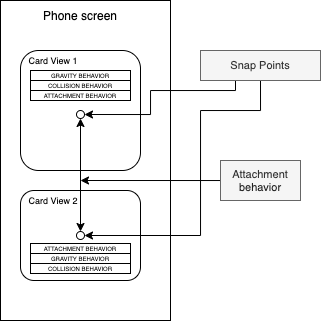
\includegraphics[width=10cm]{animation}
%     \captionof{figure}{
%        Schema dell'implementazione di UIDynamics
%     }
%     \label{fig:6}
% \end{minipage}\\

\section{Scomposizione del requisito}

Per semplicità divido il requisito in diversi punti e per ognuno ne spiego la soluzione
o metodologia utilizzata:

\begin{enumerate}
    \item\label{animationenum:1} Le animazioni devono essere disponibili in qualunque sezione o vista in cui si trovi l'utente e definite dal contesto attuale;

    \item\label{animationenum:2} Ogni CardView deve essere trascinabile dall'utente;
    
    \item\label{animationenum:3} Quando l'utente usa una forza di trascinamento superiore a un valore di soglia tutte le viste devono
        cadere per gravità;

    \item\label{animationenum:4} Ogni CardView mostrerà un contenuto dinamico differente e definito da dei componenti
    limitati specifici

    \item\label{animationenum:5} Le animazioni in questione devono essere progettate in pagine, in cui ogni pagina può contenere 
    più CardView. L'utente vedrà in un determinato momento una e soltanto una pagina. 
    Una volta che le CardView acquisisco una gravità e cadono, finirà l'animazione o apparirà
    una nuova pagina, se presente;

    \item\label{animationenum:7} Ogni CardView deve interagire con le altre della stessa pagina, come se si toccassero;

\end{enumerate}

% % % % % % % % % % % % % % % % % % % % % % % % % % % % % % % % % % % % %
%                      Onnipresenza delle animazioni                    %
% % % % % % % % % % % % % % % % % % % % % % % % % % % % % % % % % % % % %
\subsection{~\ref{animationenum:1}. Onnipresenza delle animazioni}

\textbf{Premessa}: il contenuto di ogni applicazione iOS è inserito all'interno di un oggetto denominato
\textbf{UIWindow}\cite{uiwindow}. Questa finestra è disponibile in ogni UIViewController e permette di aggiungere contenuti
come viste o interi UIViewController al di sopra di tutto il contesto dell'app. Questo rende essenzialmente ogni contenuto presentato
indipendente per esempio da un stack di navigazione.\\ 

Per creare animazioni definite dal contesto usiamo quindi un semplice UIViewController che gestirà tutte le animazioni,
ma invece di presentarlo attraverso i metodi base visti alla sezione~\ref{sec:navigation}, lo presentiamo al di sopra della UIWindow,
in modo da non essere vincolati dal contesto dell'utente quando l'animazione finirà, ma allo stesso tempo
consente di controllare l'inizializzazione di questo UIViewController in base al contesto.

% % % % % % % % % % % % % % % % % % % % % % % % % % % % % % % % % % % % %
%                        CardView trascinabile                          %
% % % % % % % % % % % % % % % % % % % % % % % % % % % % % % % % % % % % %
\subsection{~\ref{animationenum:2}. Aggiunta di una gesture}

In iOS per interagire con le viste attraverso il display touch screen si utilizzano delle UIGestureRecognizer.
Tali strumenti sono nativi e offrono diverse tipologie per l'iterazione:
\begin{itemize}
    \item UITapGestureRecognizer: respansabile della gestione dei tap

    \item UIPinchGestureRecognizer: respansabile della gestione del pitch ossia la gesture spesso usata per lo zoom
    
    \item UIRotationGestureRecognizer: respansabile della gestione delle rotazioni
    
    \item UISwipeGestureRecognizer: responsabile di uno swipe ossia un trascinamento in una direzione molto breve
    
    \item UIPanGestureRecognizer: responsabile del drag and drop
    
    \item UIScreenEdgePanGestureRecognizer: responsabile di uno swipe ossia un trascinamento nei bordi dello schermo
    
    \item UILongPressGestureRecognizer: responsabile di una prossione prolungata nel tempo
\end{itemize}

Per un'animazione che ha necessità di muoversi come se l'utente la stesse spostando occore una UIPanGestureRecognizer.
Dalla doumentazione delle UIGestureRecognizer viene spiegato che ohni vista "draggabile" necessiata una gesture,
per questo ogni card view dovrà averne una.

% % % % % % % % % % % % % % % % % % % % % % % % % % % % % % % % % % % % %
%                        Gravity                                     %
% % % % % % % % % % % % % % % % % % % % % % % % % % % % % % % % % % % % %
\subsection{~\ref{animationenum:3}. Aggiunta della gravità }

Attraveso la UIPanGesture è possibile calcolare il vettore della velocità del trascinamento,
con questo semplice dato e ciò che abbiamo studiato dello UIKit Dynamics è possibile aggiungere una gravità solo se
il vettore della velocità è superiore a una soglia prestabilita.

Per implementarlo è stato utilizzato un UIGravityBehavior, inizializzato in questo modo:

\begin{minted}{swift}
    let gravityBehavior = UIGravityBehavior(items: page.views)
    gravityBehavior.magnitude = Constants.gravity
\end{minted}

Il valore \textbf{magnitude} è la forza di gravità che vogliamo
assegnare alle viste in questione. \\

Nella figura~\ref{fig:6} si vede lo schermo di uno smartphone, che presenta l'animazione
voluta in questo caso con due CardView. Ognuna di esse ha un \textbf{UIAttachmentBehavior} al
centro per fare in modo che sia sempre centrata in esso (o nel punto di drag dell'utente),
un \textbf{UICollisionBehavior} per permettere che durante il drag le CardView possa scontrarsi e non si accavallino e un \textbf{UIGravityBehavior}, il quale 
viene utilizzato per la caduta delle viste alla fine dell'animazione o al cambiamento di pagina.

In più esiste uno speciale UIAttachmentBehavior tra i centri delle due CardView per permettere che il movimento di una
sposti anche l'altra, è una sorta di corda che le lega.

Per l'ingresso invece è stato inserito un UISnapBehavior, al centro per ogni oggetto, che anima 
gli oggenti dando un effetto a molla.

Tutte le animazione sono attivate e disattive in specifici momenti, questo dipende 
dalla UIPanGestureRecognizer e dai movimenti dell'utente.

% % % % % % % % % % % % % % % % % % % % % % % % % % % % % % % % % % % % %
%                        Modular CardView                               %
% % % % % % % % % % % % % % % % % % % % % % % % % % % % % % % % % % % % %
\subsection{~\ref{animationenum:4}. La CardView modulare}

L'intero UIViewControllor che regola le CardView animate è stato progettato per presentare 
animazioni con contenuti dinamici, per questo sono state progettate delle strutture dati specifiche per consentire la personalizzazione
del contenuto di ogni CardView. 

Inizialmente sono stati definiti i possibili componenti che ogni CardView può adottare:
\begin{itemize}
    \item\textbf{Solo testo}: Il componente include un testo, il suo colore e il colore di sfondo
    \item\textbf{Solo Immagine}: Il componente include un'immagine e il colore di sfondo
    \item\textbf{Row}: Il componente include un'icona e due testi in quest'ordine;
    \item\textbf{Animazione Lottie\cite{lottie}}: Il componente include una semplice UIView in cui viene mostrata un'animazione Lottie
    \item\textbf{Footer}: Il componente include del testo e un'icona sulla destra;
\end{itemize}

Una volta definiti tutti i componenti per ogni CardView questa viene assemblata "incollando" un componente
dopo l'altro attraveso una vista chiamata ModularCardView, di seguito, in figura~\ref{fig:7} il risultato finale ottenuto. \\

\begin{minipage}{\linewidth}
    \centering
    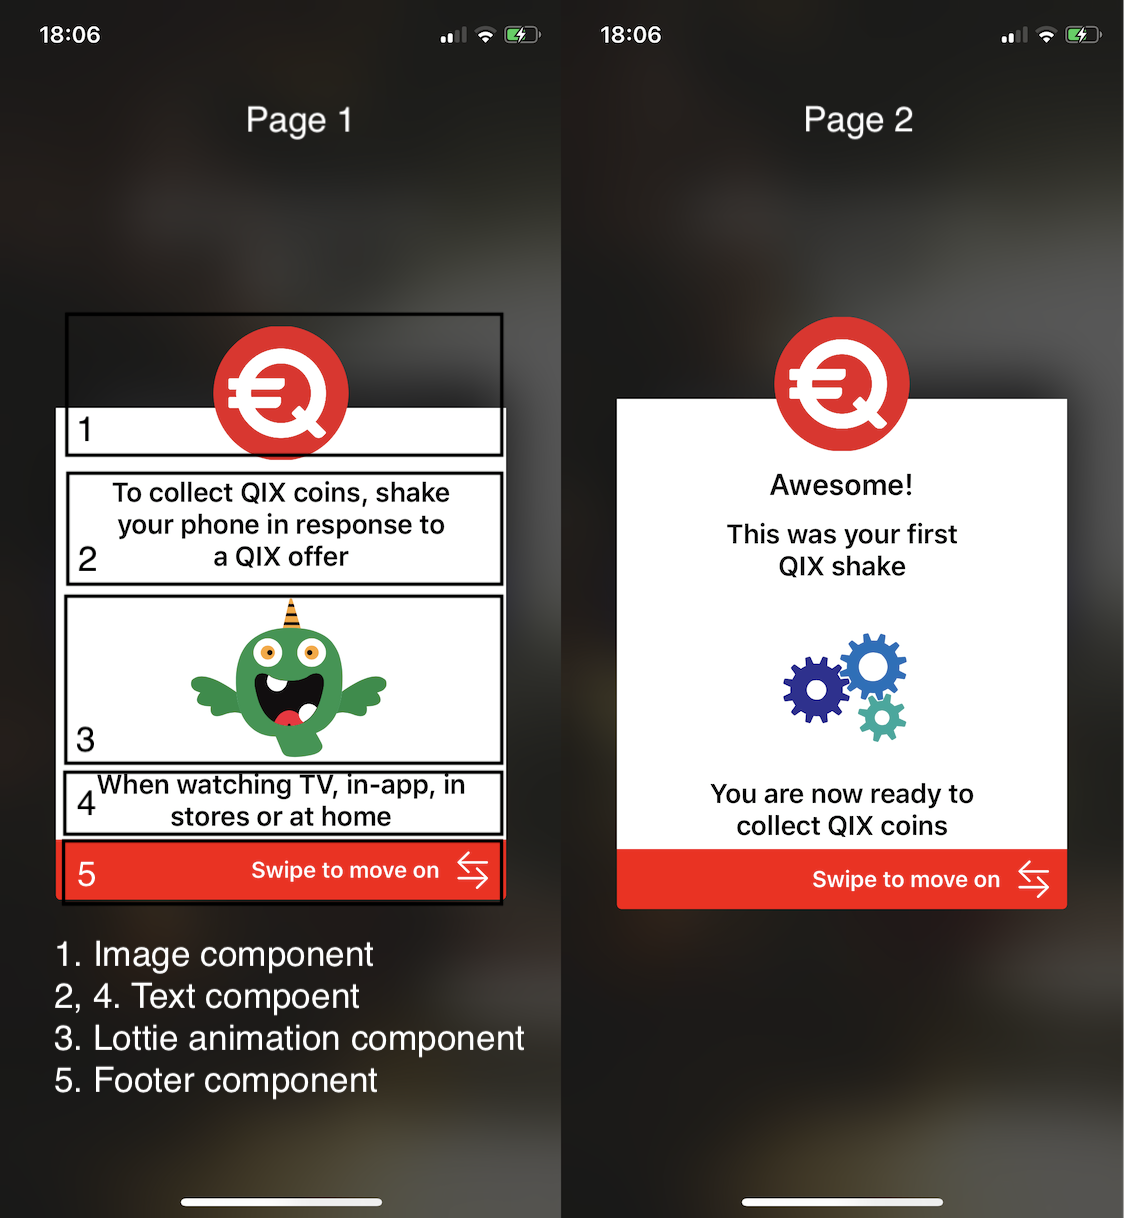
\includegraphics[width=10cm]{an12}
    \captionof{figure}{
       CardViews modulari
    }
    \label{fig:7}
\end{minipage}\\


% % % % % % % % % % % % % % % % % % % % % % % % % % % % % % % % % % % % %
%                   La paginazione delle animazioni                     %
% % % % % % % % % % % % % % % % % % % % % % % % % % % % % % % % % % % % %
\subsection{~\ref{animationenum:5}. Paginazione delle animazioni}

Avendo definito al punto~\ref{animationenum:1} l'utilizzo di un solo UIViewController per le animazioni da un lato viene semplificata
la presentazione delle stesse, dato che basterà presentare un solo UIViewController, ma dall'altro verrà delegata
l'intera paginagione al view controller. \\

In particolare questo UIViewController accetta come variabile di inizializzazione
un array di pagine e in base allo stato della UIPanGestureRecognir deciderà se passare alla pagina successiva
o interrompere l'animazione;

% % % % % % % % % % % % % % % % % % % % % % % % % % % % % % % % % % % % %
%                   La paginazione delle animazioni                     %
% % % % % % % % % % % % % % % % % % % % % % % % % % % % % % % % % % % % %
\subsection{~\ref{animationenum:5}. Il Collider}

Come accennato al punto~\ref{animationenum:3} ogni le CardView hanno dei comportamenti fisici definiti
da UIkit Dynamics, in particolare per conferire un effetto di collisione viene usato un \textbf{UICollisionBehavior} e implementato come segue:

\begin{minted}{swift}
    let itemsCollisionBehavior = UICollisionBehavior(items: page.views)
\end{minted}

In questo modo ogni ogni oggetto con questo
comportamento riuscirà a scontrasi con gli altri oggetti simili.
